\documentclass{beamer}

\usepackage[ngerman]{babel}
\usepackage[utf8]{inputenc}
\usepackage{listings}
% this makes < > work
\usepackage[T1]{fontenc}
\usepackage{graphicx}
\usepackage{caption}
\usepackage{subcaption}

\lstset{
    language=c++,
    basicstyle=\tiny,
    showspaces=false,
    showstringspaces=false
}
\setbeamertemplate{footline}{\insertframenumber/\inserttotalframenumber}

\title{Using CGAL to create Apollonius diagrams based on OpenStreetMap data}

\author[Sebastian Kürten, Philipp Borgers, Lukas Maischak]{
    Sebastian Kürten
    \newline Lukas Maischak
    \newline Philipp Borgers
}

\begin{document}

\begin{frame}
    \titlepage
\end{frame}

\begin{frame}
    \frametitle{Thema}
    \begin{itemize}
        \item Approximation von Gemeindegrenzen mit Hilfe von Apollonius-Diagrammen
        (Additiv gewichtete Voronoi-Diagramme)
        \item Datenbasis: sogenannte Ortsknoten aus der Openstreetmap Datenbank
        \item Eingabe: Menge von Knoten mit Metadaten (Einwohnerzahl)
        \item Ausgabe: Zu jedem Knoten konstruiere ein Polygon, welches die der Gemeinde
        zugeordnete Fläche bestimmt.
        \item Dabei sollen die Polygone eine Zerlegung der Ebene bilden.
    \end{itemize}
\end{frame}

\begin{frame}
    \frametitle{Apollonius diagram (2D)}
    \begin{itemize}
        \item aka. additively weighted Voronoi diagram
        \item Subdivision of the plane into connected regions (cells)
        \item Defined over a set of sites $P_i = (c_i, w_i)$
        \item A cell contains all points that are closer to $P_i$ than to any
            other site $P_j$
    \end{itemize}
\end{frame}

\begin{frame}
    \frametitle{Apollonius graph}
    \begin{itemize}
        \item The dual of the Apollonius diagram
    \end{itemize}
\end{frame}

\begin{frame}
    \frametitle{Examples in 2D}
    \begin{figure}[htp]
            \centering
            \begin{subfigure}[b]{0.48\textwidth}
                    \centering
                    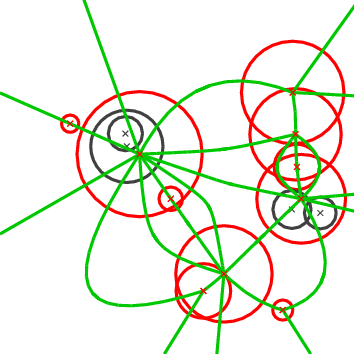
\includegraphics[width=\textwidth]{../final-report/images/apollonius-graph.png}
                    \caption{Apollonius graph}
                    \label{fig:apo-graph}
            \end{subfigure}
            \begin{subfigure}[b]{0.48\textwidth}
                    \centering
                    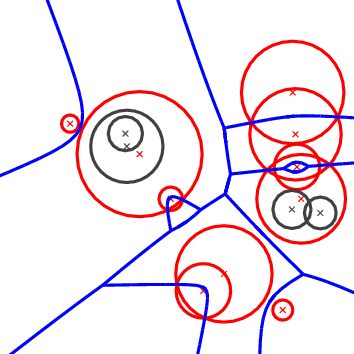
\includegraphics[width=\textwidth]{../final-report/images/apollonius-diagram.png}
                    \caption{Apollonius diagram}
                    \label{fig:apo-diagram}
            \end{subfigure}
            \caption{Apollonius graph and Apollonius diagram}\label{fig:apollonius}
    \end{figure}
\end{frame}


\begin{frame}
    \frametitle{CGAL Apollonius graph}
    \lstinputlisting{../final-report/code/init-apollonius-graph.c}
\end{frame}

\begin{frame}
    \frametitle{CGAL Implementierung - Dual Graph}
    \begin{itemize}
        \item How we generate the graph
    \end{itemize}
\end{frame}

\begin{frame}
    \frametitle{Vorverarbeitung}
    \begin{itemize}
        \item Extract place nodes (city, town, village) from OpenStreetMap dataset 
        \item Use the position information and the osm-id for later reference
        \item Format: <Openstreetmap Node Id> <Longitude> <Latitude> <type>
    \end{itemize}
\end{frame}

\begin{frame}
    \frametitle{Output-Formats: WKT}
    \lstinputlisting{../final-report/code/output.wkt}
\end{frame}

\begin{frame}
    \frametitle{Output-Formats: WKT}
    \lstinputlisting{../final-report/code/wkt.c}
\end{frame}

\begin{frame}
    \frametitle{Output-Formats: GeoJSON}
    \lstinputlisting{../final-report/code/output.json}
\end{frame}

\begin{frame}
    \frametitle{Output-Formats: GeoJSON}
    \lstinputlisting{../final-report/code/geojson.c}
\end{frame}

\begin{frame}
    \frametitle{Output-Formats: SQL}
    \lstinputlisting{../final-report/code/output.sql}
\end{frame}

\begin{frame}
    \frametitle{Output-Formats: SQL}
    \lstinputlisting{../final-report/code/sql.c}
\end{frame}

\begin{frame}
    \frametitle{Demo}
    \begin{center}
        Ludi incipiant
    \end{center}
\end{frame}

\begin{frame}
    \frametitle{Questions?}
    \begin{center}
    Questions?
    \newline Thank you for your attention!
    \end{center}
\end{frame}

\begin{frame}
    \frametitle{Sources}
    \begin{itemize}
        \item foo
    \end{itemize}
\end{frame}

\end{document}
